\section{基本概念与核心特点}

\subsection{定义与数学基础}
图论是图数据库的理论基础, 如\cref{fig:graph}所示. 图是由一组节点和连接这些节点的边组成的数学结构. 在图数据库中, 实体的每个特征可以作为节点的属性进行存储, 关系也可以具有属性. 这种方式使得图数据库能够直观地反映出实体之间的各种关系, 并通过图遍历等算法快速进行数据查询.

\begin{figure}[H]
	\centering
	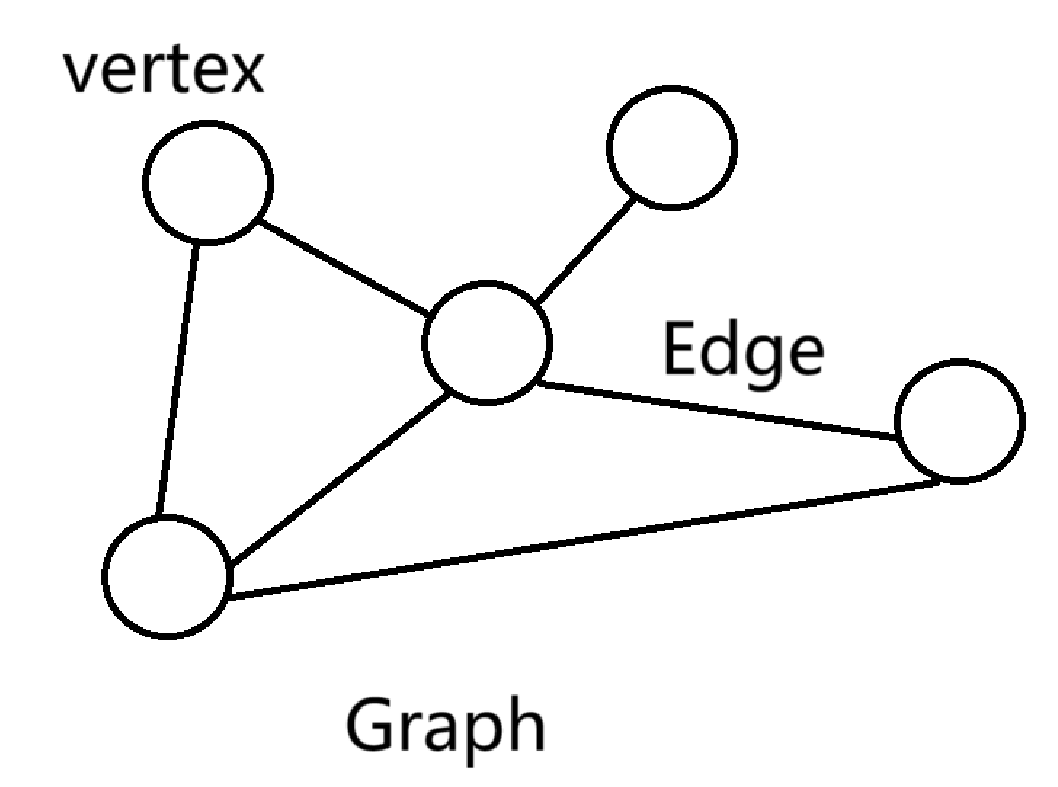
\includegraphics[width=1\textwidth]{images/7.png}
	\caption{数学上的图}
	\label{fig:graph}
\end{figure}
图数据库是一种用于管理和存储图结构数据的数据库管理系统, 以图论为理论基础进行数据建模. 图数据库中的基本单位是“节点 (Vertex) ”和“边 (Edge) ”, 其中节点用于表示实体, 边用于表示实体之间的关系. 与关系型数据库不同, 图数据库直接存储数据中的关系, 使得其能够更加自然和高效地表示复杂的数据结构. 例如, \cref{fig:social-network}展示了一个简单的社交网络图, 其中节点代表用户, 边代表用户之间的好友关系. 图数据库能够直观地表示这种复杂的关系, 并通过图遍历等算法快速进行数据查询, 从而实现商品推荐,社区发现等上层应用.
\begin{figure}[H]
	\centering
	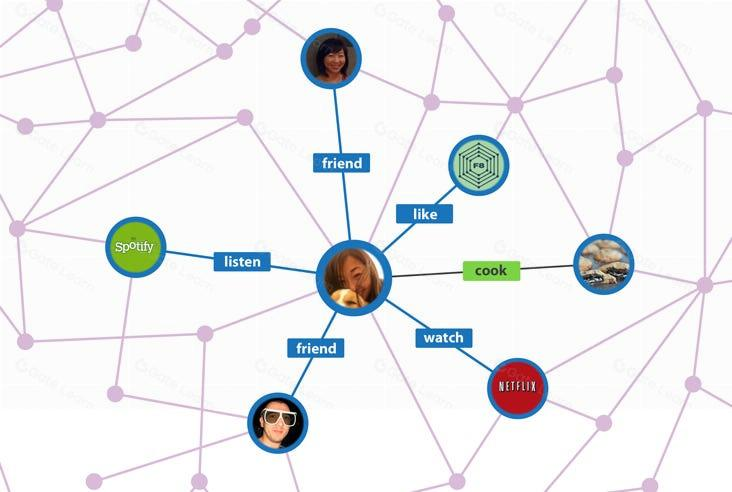
\includegraphics[width=0.8\textwidth]{images/8.png}
	\caption{社交网络}
	\label{fig:social-network}
\end{figure}


\subsection{主要模型}

图数据库主要有三种模型:

\textbf{属性图模型:} 属性图模型是图数据库中最常见的模型, 如\cref{fig:property-graph}所示,其特点是节点和边都可以附带多个属性 (键值对) , 便于对复杂关系进行建模. 例如, 在社交网络中, 节点可以代表用户, 边可以代表好友关系, 而属性则可以存储用户的年龄或好友关系的建立时间. 属性图模型的优点是灵活且直观, 适合表示复杂的实体和关系, 查询效率高. 但其对于高度结构化的数据, 可能没有关系型数据库的存储和处理效率高.
\begin{figure}[H]
	\centering
	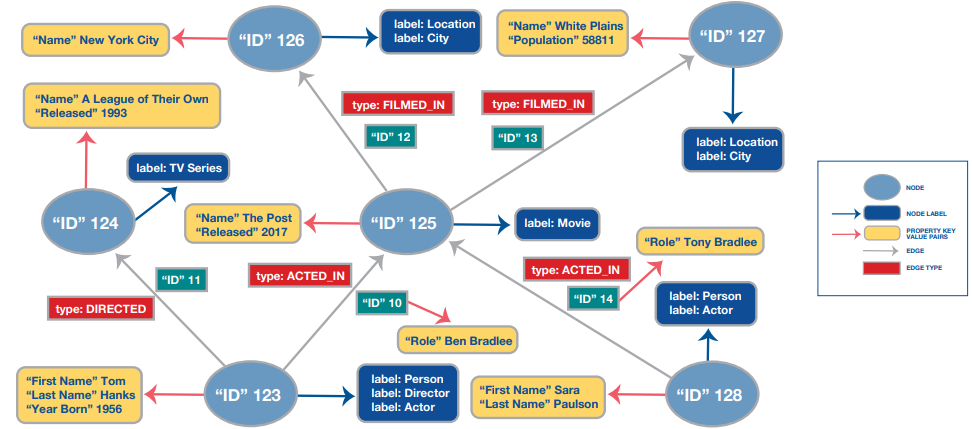
\includegraphics[width=\textwidth]{images/9.png}
	\caption{属性图模型}
	\label{fig:property-graph}
\end{figure}

\textbf{资源描述框架模型:} 资源描述框架(Resource Description Framework, RDF) 模型基于W3C提出的标准, 适用于语义网络应用. 如图\cref{fig:rdf}, 它使用三元组 (主语-谓语-宾语) 来表示数据. 例如, “Alice 是 Bob 的好友”可以表示为一个三元组. 这种模型广泛应用于语义网和知识图谱中. RDF模型的优点在于标准化程度高, 特别适合构建可扩展的语义网络, 数据互操作性好;但是其存储结构较为冗长, 对于复杂关系的查询性能可能不如属性图模型高.
\begin{figure}[H]
	\centering
	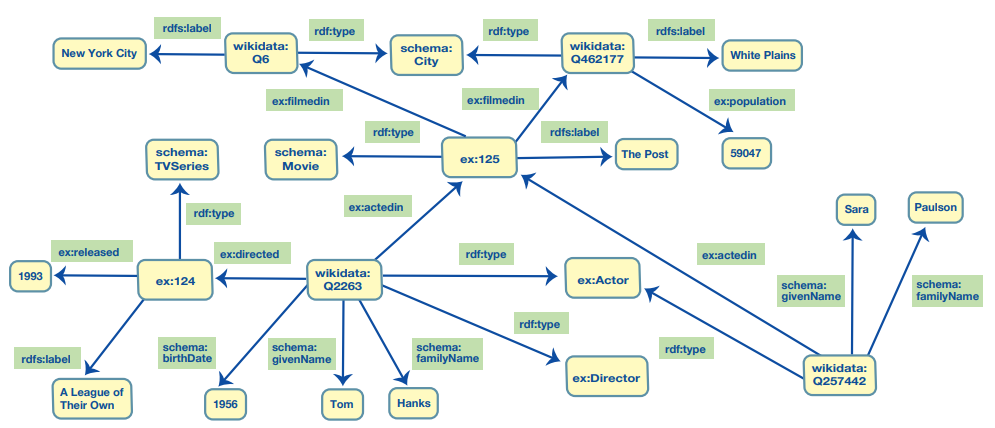
\includegraphics[width=\textwidth]{images/10.png}
	\caption{资源描述框架模型}
	\label{fig:rdf}
\end{figure}

\textbf{超图模型:} 超图是节点与一组节点之间关系的扩展, 适用于表示复杂多方关系的场景. 例如, 如\cref{fig:hypergraph1}所示,在房产证上张三与李四共同拥有三套房,在超图中就只需一条超边(拥有)就能表示出来。 但现实中,仅仅一条超边来表示拥有关系,可能会隐藏很多细节,例如房产证中每套房张三、李四各自占有的比率,因此,如果用属性图来表示将更为丰富,只是将一条超边转化, 为6条属性图中的关系,如\cref{fig:hypergraph2}所示。 超图模型的优点是能够更加方便地表示多对多的关系, 适合描述复杂的群体交互场景;但其实现复杂度较高, 查询操作也可能比其他图模型更加复杂, 导致查询效率受到影响.
\begin{figure}[H]
	\centering
	\begin{subfigure}[b]{0.45\textwidth}
		\centering
		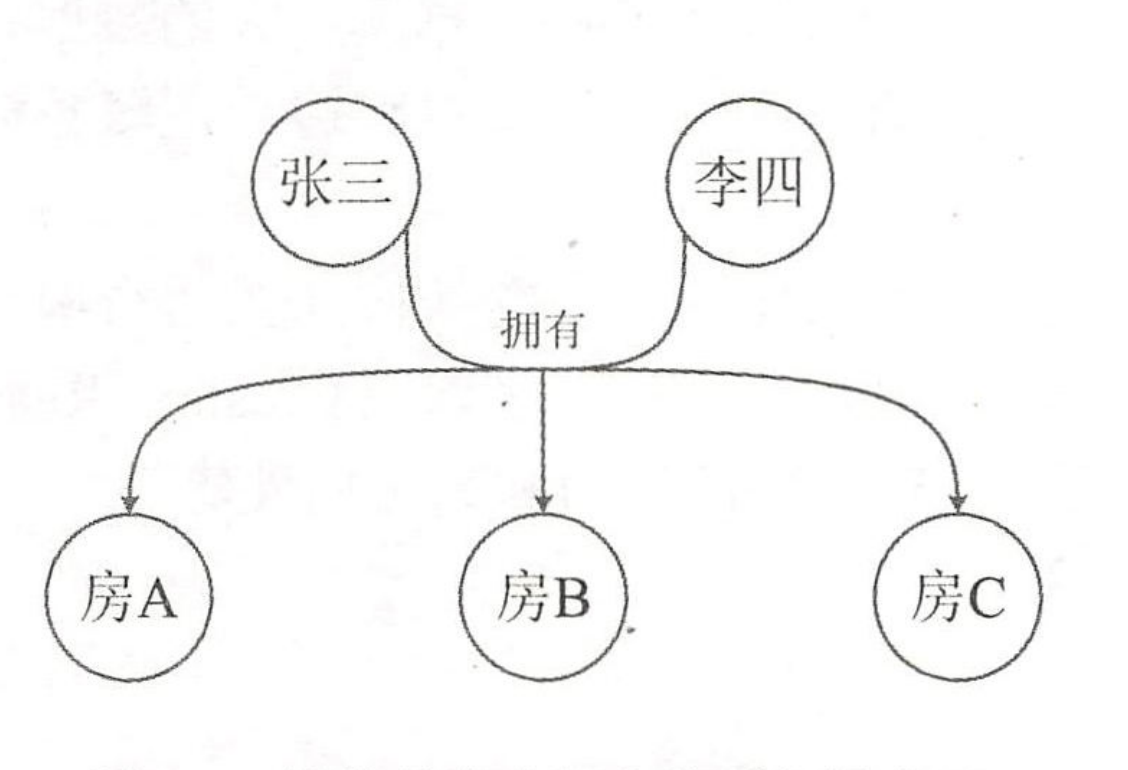
\includegraphics[width=1\textwidth]{images/16.png}
		\caption{超图模型示例1}
		\label{fig:hypergraph1}
	\end{subfigure}
	\begin{subfigure}[b]{0.45\textwidth}
		\centering
		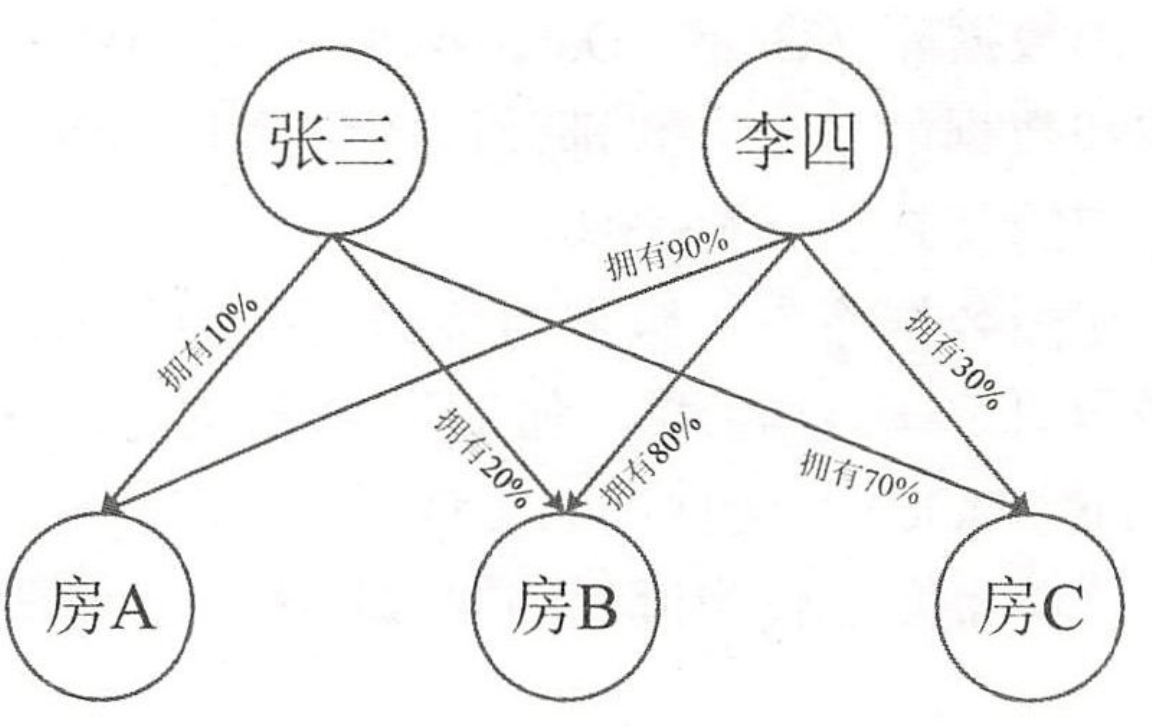
\includegraphics[width=1\textwidth]{images/17.png}
		\caption{超图模型示例2}
		\label{fig:hypergraph2}
	\end{subfigure}
	\caption{超图模型}
	\label{fig:hypergraph}
\end{figure}



\subsection{与关系型数据库的比较}

图数据库与传统关系型数据库相比, 具有显著的特点和优势.

\textbf{建模方式:} 关系型数据库使用“表格化结构”来表示数据, 适合处理结构化数据. 但当数据之间存在复杂的多层次关联关系时, 需要使用外键进行多次表连接, 导致查询效率下降. 而图数据库通过“节点-边”的建模方式, 可以更自然地表达复杂的关联关系.
\begin{figure}[H]
	\centering
	\begin{subfigure}[b]{0.45\textwidth}
		\centering
		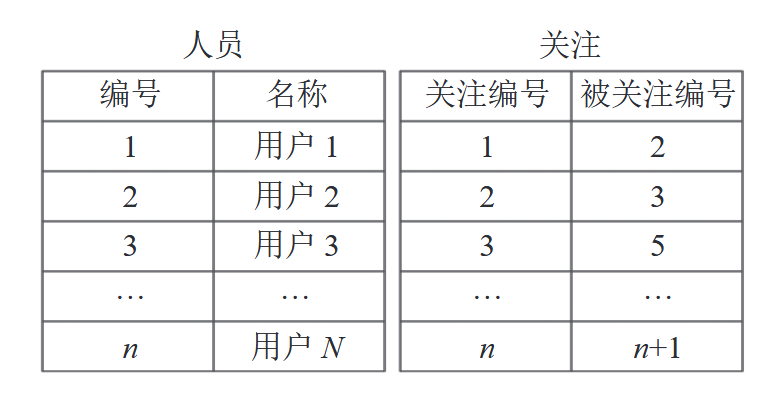
\includegraphics[width=\textwidth]{images/1.png}
		\caption{关系型数据库}
	\end{subfigure}
	\hfill
	\begin{subfigure}[b]{0.45\textwidth}
		\centering
		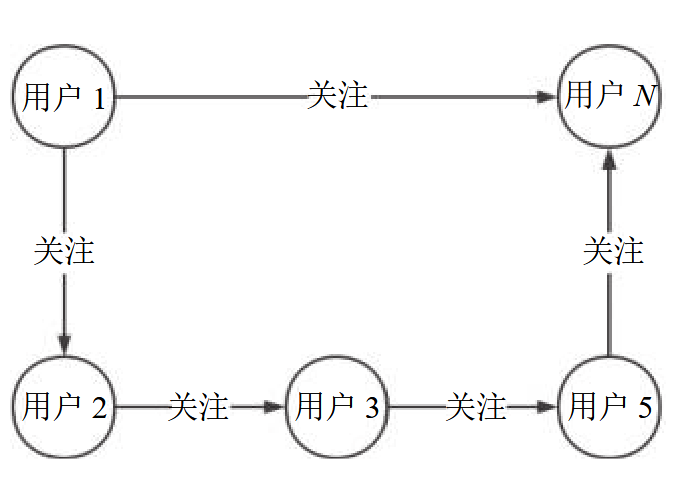
\includegraphics[width=\textwidth]{images/2.png}
		\caption{图数据库}
	\end{subfigure}
\end{figure}


\textbf{查询效率:} 在涉及深度关联的查询中, 关系型数据库需要通过多次JOIN操作进行表的关联, 查询的复杂度和时间消耗迅速增加. 而图数据库则可以通过图遍历的方式, 直接在节点和边之间进行跳转, 大幅提高查询效率.

\textbf{灵活性:} 图数据库具有灵活的数据模式, 支持在不影响现有数据的情况下对数据模型进行扩展. 这种灵活性使得图数据库在面对动态变化的数据结构时, 能够更轻松地进行更新和维护.
